\documentclass[tikz, dvipdfmx]{standalone}
\usepackage{tikz}

\usetikzlibrary{intersections,calc,arrows.meta}
\begin{document}
  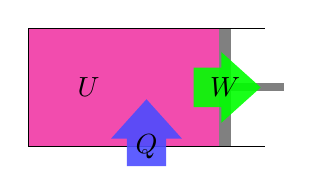
\begin{tikzpicture}
    \begin{scope}[scale = 0.5]
    \fill[magenta, opacity=0.7] (-3,-1.5) rectangle (1.85,1.5);
    \fill[gray] (1.85,1.5) rectangle (2.15,-1.5);
    \fill[gray] (2.1,0.1) rectangle (3.5,-0.1);
    \draw[line width=0.5pt] (3,1.5) -- (-3,1.5) -- (-3,-1.5) -- (3,-1.5);
    \fill[blue!70!white, opacity=0.9] (0,-0.3) -- (0.9,-1.3) -- (0.5,-1.3) -- (0.5,-2) -- (-0.5,-2) -- (-0.5,-1.3) -- (-0.9,-1.3) --cycle;
    \fill[green, opacity=0.9] (1.2,0.5) -- (1.2,-0.5) --(1.9,-0.5) -- (1.9,-0.9) -- (2.9,0) --(1.9,0.9) -- (1.9,0.5) -- cycle;
    \end{scope}
    \draw (-1,0) node[right]{$U$};
    \draw (0,-0.75) node{$Q$};
    \draw (1,0) node{$W$};
  \end{tikzpicture}
\end{document}
